\section{Functional Interpretation of LLM Exploration Behavior}

\begin{figure*}[h]
\centering
\begin{subfigure}[t]{\textwidth}
\centering
\caption{\textbf{MAB} in Easy ($K$=5, $\Delta_{\min}$=0.5).}
% \vspace{-24mm}
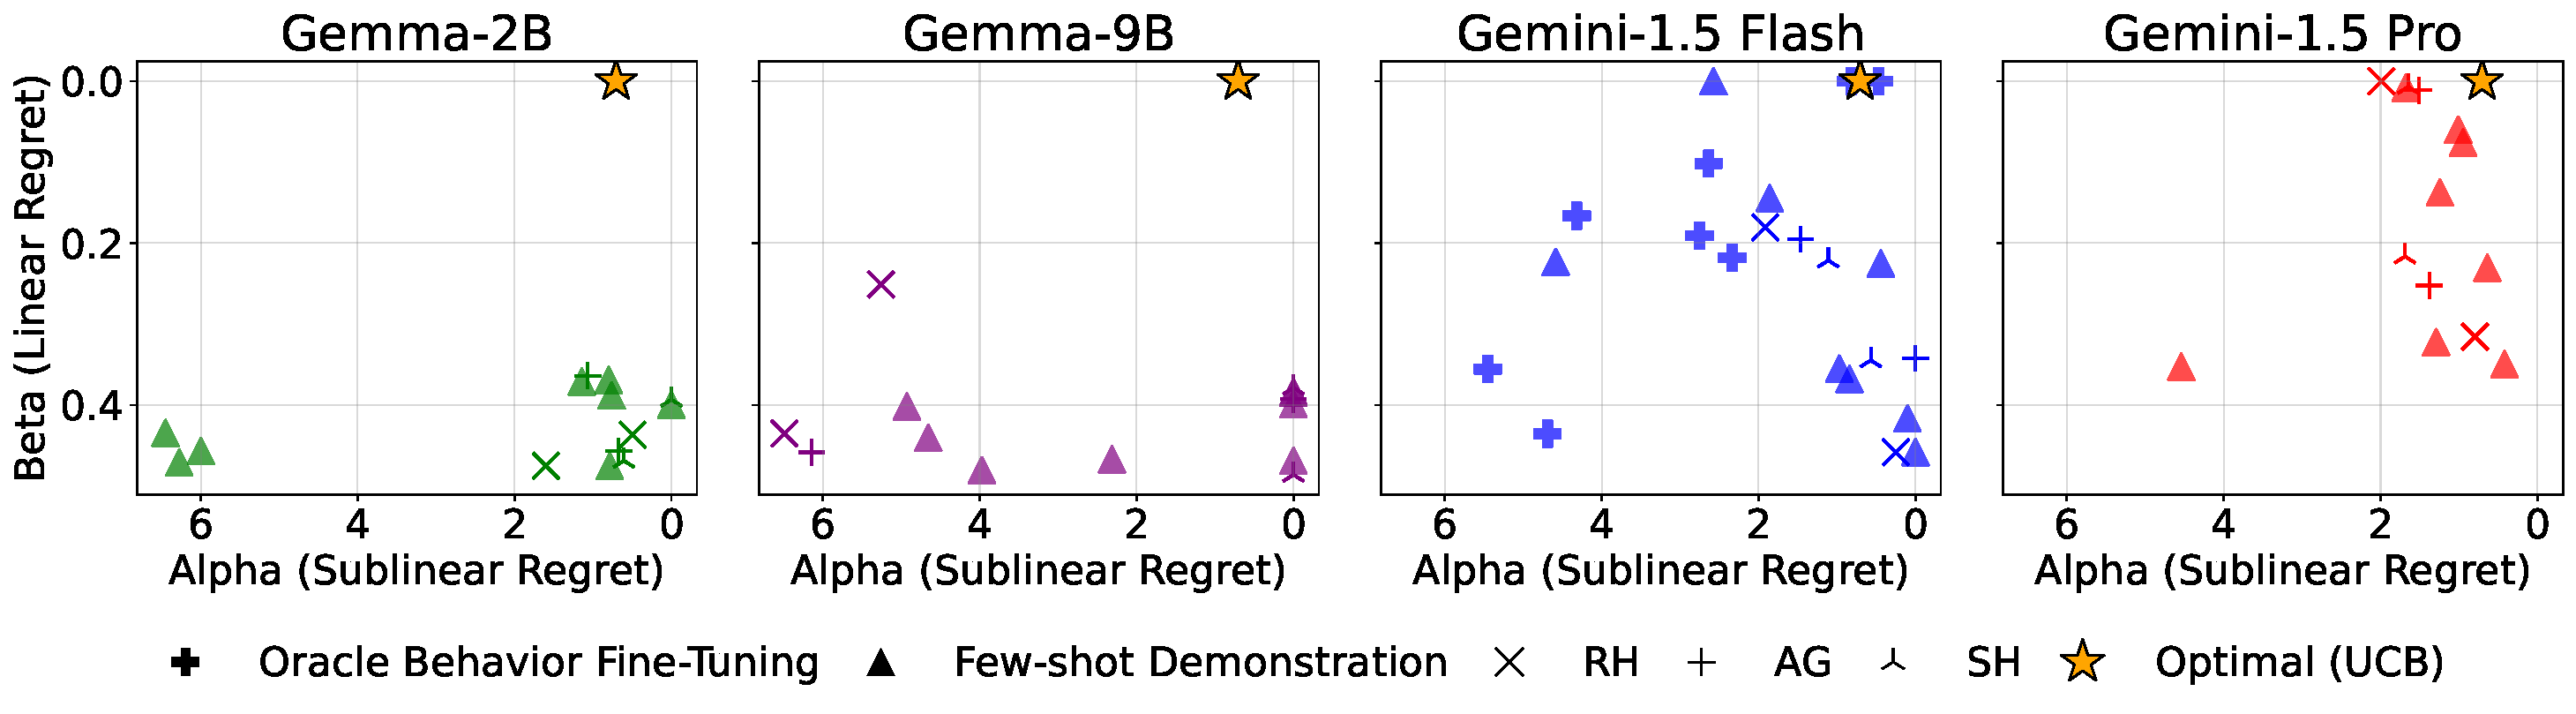
\includegraphics[width=\textwidth]{figures/mab_easy_domain_exp_multi.pdf}
\label{fig:exp_analysis_easy}
\end{subfigure}
\quad
\begin{subfigure}[t]{\textwidth}
\centering
% \vspace{-24mm}
\caption{\textbf{MAB} in Hard ($K$=20, $\Delta_{\min}$=0.2).}
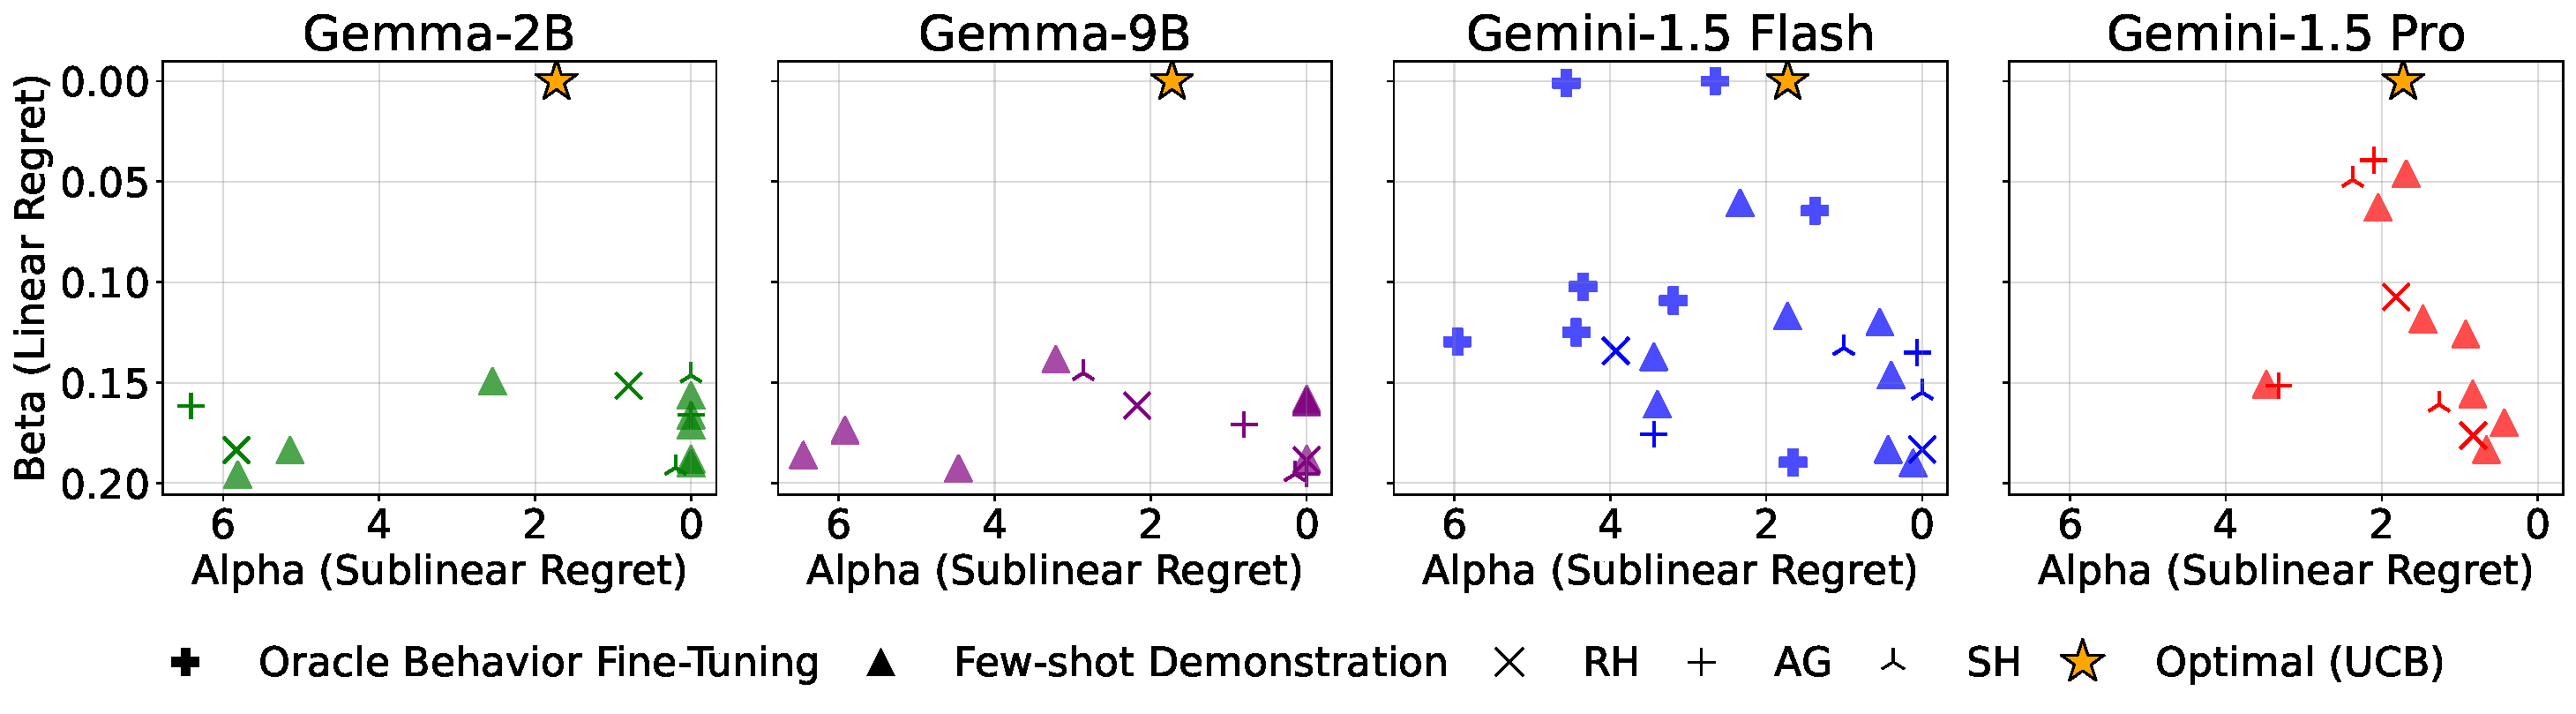
\includegraphics[width=\linewidth]{figures/mab_hard_domain_exp_multi.pdf}
\label{fig:exp_analysis_hard}
\end{subfigure}
\centering 
\caption{\footnotesize{We plot the estimated parameters $\alpha$ and $\beta$. Smaller $\alpha$ and $\beta$ indicate more efficient exploration to find the best arm. Algorithms with strong in-context exploration should have $\alpha$ as small as possible and have $\beta$=0. We can see for MAB Hard setup, lesser models achieved sublinear regret.}}
\label{fig:exp_analysis}
\vspace{-4mm}
\end{figure*}

In this section, we aim to conduct a more rigorous analysis of the LLM's exploration efficiency using the concept of regret, $REG(\pi)$. Most bandit algorithms are evaluated by the behavior of $REG(\pi)$ as a function of $T$ (i.e., the number of interactions), either theoretically or empirically. 
Motivated by this, our goal is to understand the exploration behaviors of various LLMs by characterizing their regret as a function of $T$. To achieve this, we adopt the following functional form to analyze the regret:
\begin{align}
 f(T) = \frac{\lambda \log(T)^{\alpha}}{\Delta_{\min}} + \beta T + \lambda_2
\end{align}
The three parameters $\alpha, \beta, \lambda_1$ in the equation are all positive real numbers. $\lambda_2$ is unconstrained. $\Delta_{\min}$ captures the gap between the best and second best arm.
This functional form provides intuitive interpretations for the underlying parameters. Specifically, $\log(T)$ represents sublinear scaling of the regret, which is known to be achieved by only the best bandit algorithms (e.g. UCB and Thompson Sampling). The $T$ scaling describes a linear growth or the inability of an agent to match the optimal policy $\pi^*$. This means a strong algorithm should have $\alpha$ as small as possible, and have $\beta=0$. This functional form also allows us to see some growth behaviors in-between with both positive $\alpha$ and $\beta$.
% that is not fully concave yet not fully linear because the function can have both $\alpha$ and $\beta$ to be non-zero to blend a concave function and a linear function together.
We use the curve fit function in Scikit-learn~\citep{pedregosa2011scikit} to fit the cumulative regret curve of UCB and LLMs coupled with different methods (i.e., inference-time algorithm-guided support, in-context demonstration, and optimal behavior fine-tuning).
The results of the fitted $\alpha$ and $\beta$ values are presented in Figure~\ref{fig:exp_analysis}. 
For the largest Pro models, applying effective inference-time support, such as \textbf{AG} and \textbf{SH} can achieve nearly sub-linear regret. More intriguingly, for Flash models, fine-tuning for optimal behavior significantly boosts performance, enabling them to attain sub-linear regret with a lower $\alpha$. In contrast, weaker models such as Gemma 2B and 9B appear to remain in the linear regret regime across nearly all methods.
